\documentclass[conference]{IEEEtran}
\IEEEoverridecommandlockouts
% The preceding line is only needed to identify funding in the first footnote. If that is unneeded, please comment it out.
\usepackage{cite}
\usepackage{amsmath,amssymb,amsfonts}
\usepackage{algorithmic}
\usepackage{graphicx}
\usepackage{url}
\usepackage[utf8]{inputenc}
\usepackage{textcomp}
\usepackage{multirow}
\usepackage{booktabs}
\usepackage{subfig}
\usepackage{nameref}

\usepackage[english,ngerman,brazilian]{babel}
\def\BibTeX{{\rm B\kern-.05em{\sc i\kern-.025em b}\kern-.08em
    T\kern-.1667em\lower.7ex\hbox{E}\kern-.125emX}}
\begin{document}

\title{PD5 - Reconhecimento de Objetos}

\author{\IEEEauthorblockN{Frederico Guth (18/0081641)}
\IEEEauthorblockA{\textit{Tópicos em Sistemas de Computação, ,} \\
\textit{Turma TC - Visão Computacional (PPGI)}\\
\textit{Universidade de Brasília}\\
Brasília, Brasil\\
fredguth@fredguth.com}
}

\maketitle

\begin{abstract}
Reconhecimento de Objetos lida com a identificação de objetos em imagens. Técnicas baseadas em \textit{deep learning} têm sido as mais bem sucedidas para este problema. Neste projeto, classificamos objetos da base Caltech 101\cite{caltech101} usando uma rede ResNet-50 pré-treinada e aplicamos diversas técnicas (validação cruzada, aumento de dados, otimização de taxa de aprendizado, otimizações em tempo de teste) para melhorar os resultados. Usando apenas 5 imagens de treinamento por classe, obtivemos acurácia de 85,13\%, um resultado apenas 9\% menor que o recorde para essa base, que usa 30 imagens de treinamento. 
\end{abstract}

\begin{IEEEkeywords}
reconhecimento de objetos, ResNet-50, Caltech 101, tranferência de conhecimento, cyclical learning rate
\end{IEEEkeywords}

\section{Introdução}

Reconhecimento de Objetos lida com a identificação de objetos em imagens. Quando vemos uma imagem, podemos facilmente identificar objetos, pessoas, lugares; mas algo tão natural para nós é uma tarefa bastante complexa para um algoritmo e, até pouco tempo, com resultados nada animadores.

O momento crucial no crescimento meteórico do interesse por \textit{deep learning} se deu em 2012, justamente na maior competição de reconhecimento de objetos, a  \textit{ImageNet Large Scale Visual Recognition Challenge}  (ILSVRC)\cite{goodfellow}. O time liderado por Alex Krizhevsky foi o primeiro a usar redes neurais convolucionais profundas (RCPs) na competição e ganhou por larga margem\cite{alexnet}. Desde então, técnicas baseadas em RCPs tem sido as mais bem sucedidas para este problema.


\subsection{Objetivo}
O objetivo deste projeto é propor e avaliar um método de reconhecimento de objetos para a base de imagens CalTech-101\cite{caltech101}, com apenas 5 imagens de treinamento. 

\section{Revisão Teórica}

\subsection{Redes Neurais Convolucionais Profundas}
Redes Neurais Convolucionais são modelos computacionais inspirados na biologia do cortex visual. O cortex visual tem pequenas regiões de células sensíveis a regiões específicas do campo visual\cite{hinton}.  Da mesma forma, nas RCPs filtros são convolucionados em camadas gerando novas camadas que representam onde o filtro "sensibilizou" a entrada. 

A ideia é resolver o problema da representação do conhecimento introduzindo representações que são expressas em termos de outras representações mais simples\cite{goodfellow}. Em essência, um RCP é apenas uma função matemática que mapeia um conjunto de valores de entrada a valores de saída, formada pela composição de várias funções mais simples.  Com um número suficiente de composições, camadas, é possível obter funções de alta complexidade\cite{hinton, goodfellow}. 


% \begin{figure}[ht!]
% \begin{center}
% 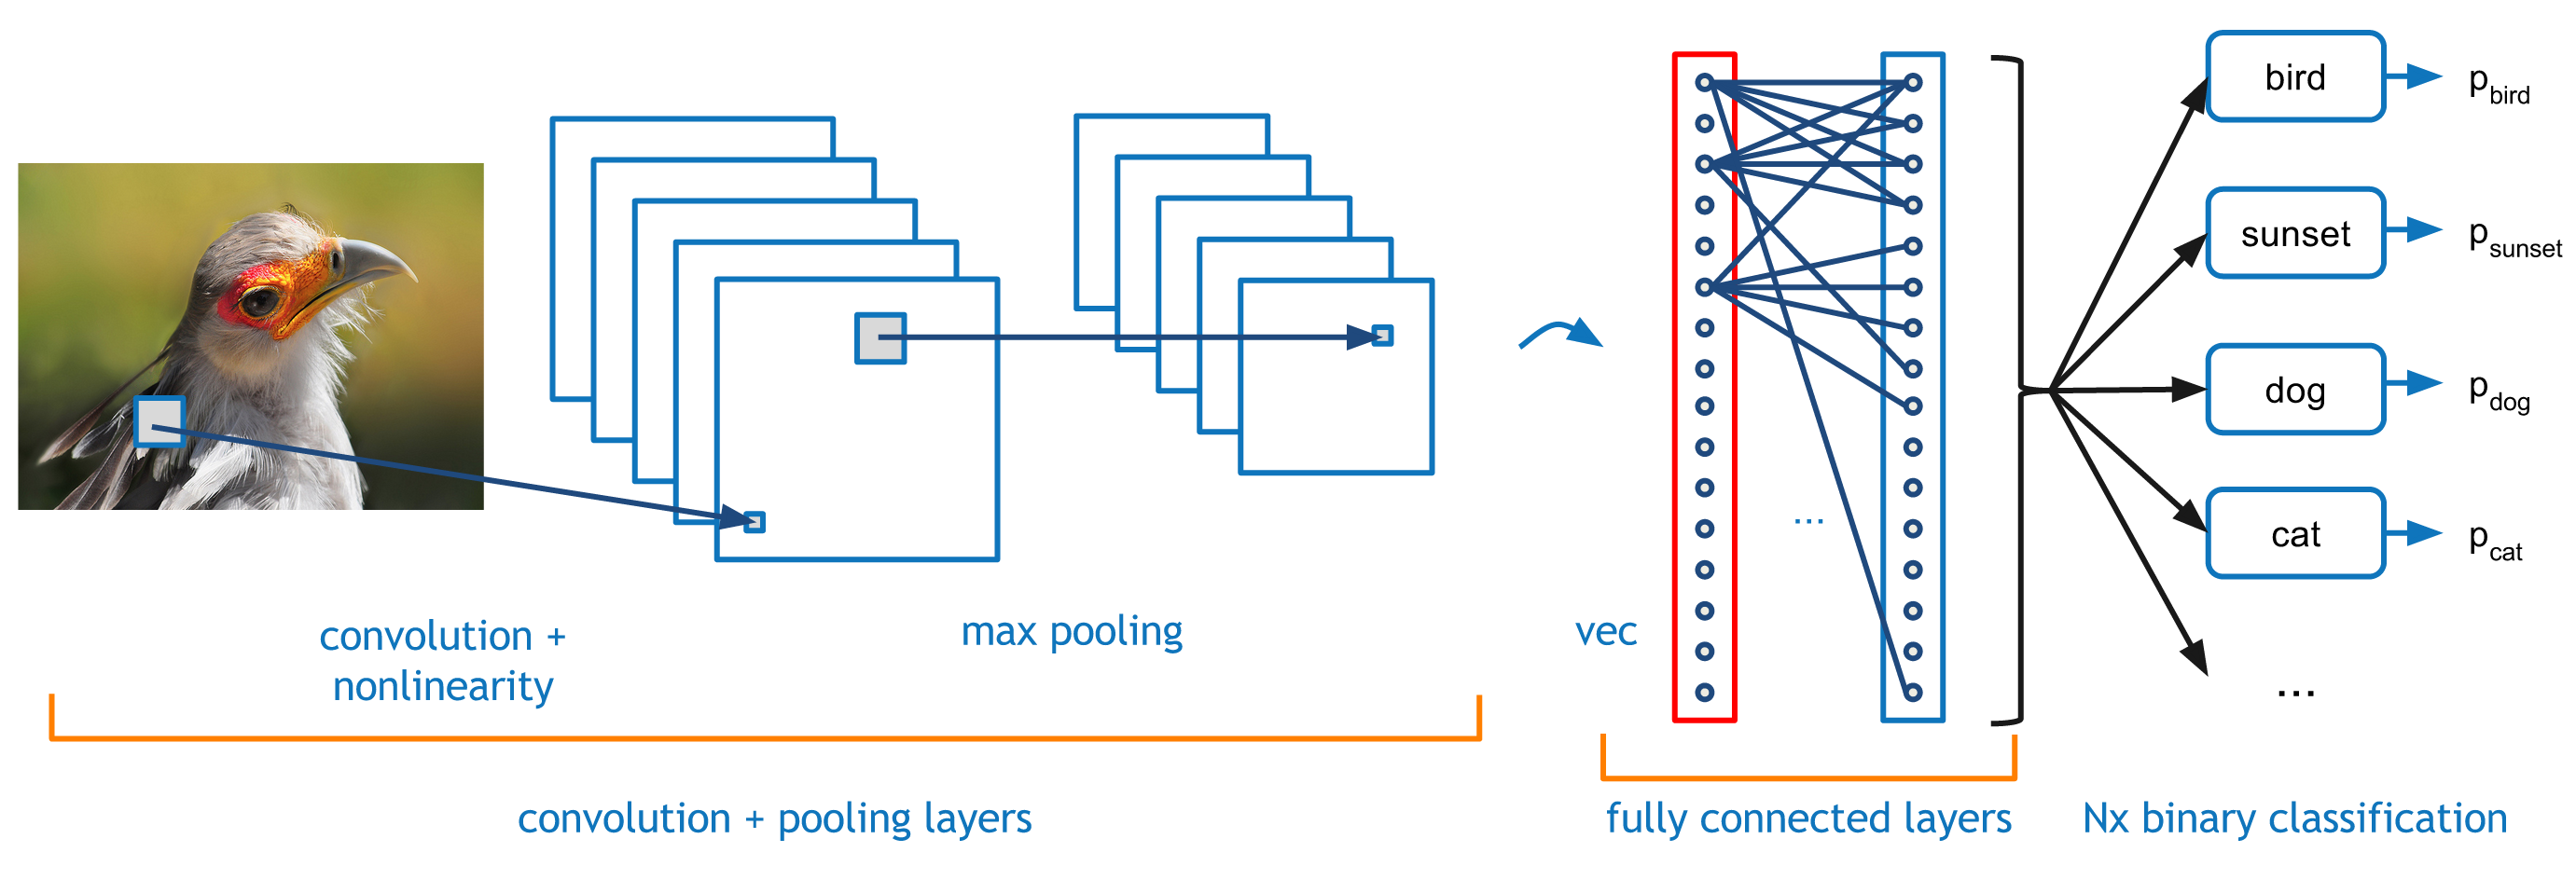
\includegraphics[width=\columnwidth]{RCP.png}
% \caption{Uma rede neural convolucional profunda}
% \end{center}
% \end{figure}
\begin{figure}[ht!]
\begin{center}
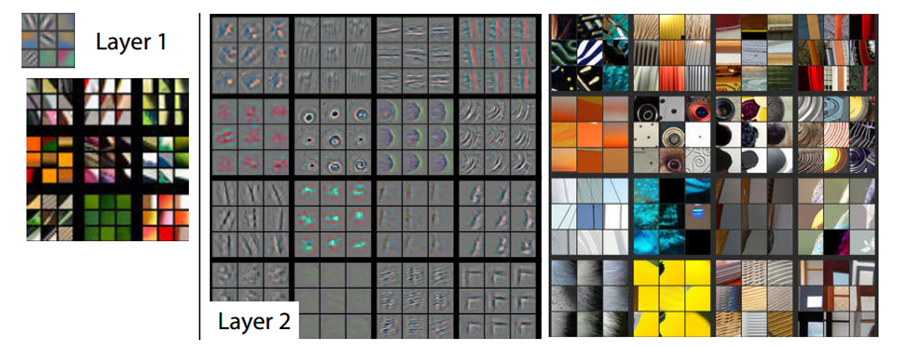
\includegraphics[width=\columnwidth]{layers.png}
\caption{Visualização de caracteríticas em um modelo já treinado\cite{zeiler}}
\label{layers}
\end{center}
\end{figure}

Em tarefas de classificação, as camadas amplificam características da entrada que são importantes para discriminação das amostras e suprimem variações irrelevantes. Uma imagem, entra como um tensor de valores de pixel,  a primeira camada tipicamente representam a presença ou ausência de bordas em determinadas orientações e localizações na imagem. A segunda, detecta padões simples e arranjos de bordas (vide Figura \ref{layers}). A terceira pode compor os padrões simples em combinações maiores que correspondem com partes de objetos, as camadas subsequentes irão detectar objetos como combinações dessas partes\cite{hinton}.


\subsection{Transferência de Conhecimento}
Em nosso dia a dia, transferimos conhecimento a todo momento. Aprender a tocar piano, facilita aprender tocar órgão. Reconhecer maçãs talvez ajude a reconhecer peras. Pessoas conseguem inteligentemente aplicar conhecimento prévio para resolver novos problemas com maior eficácia e eficiência\cite{sinno} E algoritmos?

Pesquisa em transferêcia de conhecimento tem atraído mais e mais atenção desde 1995, quando foi tema de  um workshop na NIPS-95 que discutiu a necessidade de métodos de aprendizado de máquina que retém e reusam conhecimento previamente obtido\cite{sinno}. 

No contexto de RCPs para reconhecimento visual de objetos, fica claro que as camadas iniciais: capazes de reconhecer bordas, padrões e partes de objetos, treinadas com um conjunto de imagens para reconhecer determinados rótulos (Figura \ref{layers}), podem ser usadas em outro conjunto de imagens totalmente diferente ainda que os rótulos também sejam diferentes. A capacidade de utilizar os pesos resultantes de treinamentos com milhões de imagens representa uma grande economia de processamento e uma ferramenta muito útil. 


\subsection{Hiperparâmetros}
O aspecto fundamental do \textit{deep learning} é que as camadas de características não são extraídas manualmente por pessoas; elas são aprendidas a partir dos dados usando procedimentos de aprendizados genéricos. Como consequência, RCPs podem ser retreinadas para diferentes tarefas de reconhecimento e classificação, permitindo-se aproveitar redes pré-existentes. 
% \begin{figure}[ht!]
% \begin{center}
% 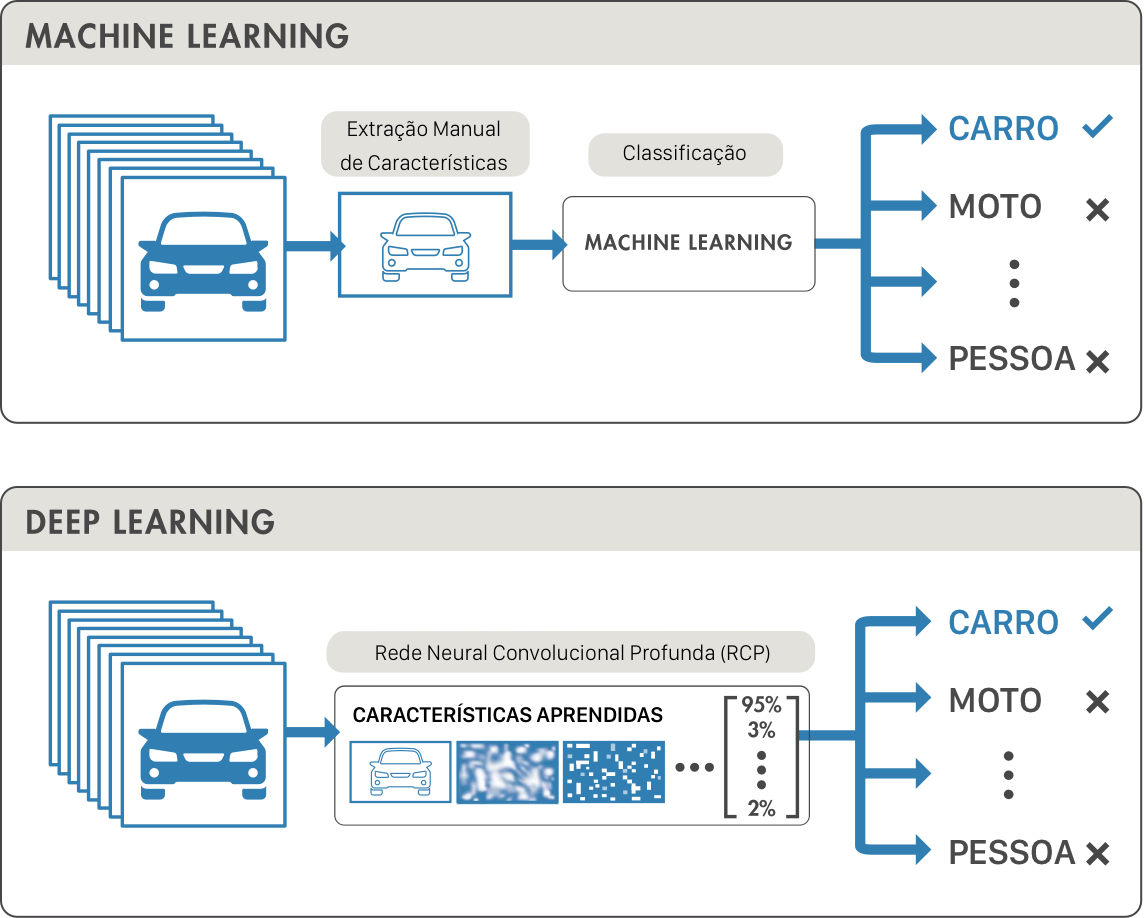
\includegraphics[width=.45\columnwidth]{MLvsDL.png}
% \caption{Machine Learning versus Deep Learning}
% \end{center}
% \end{figure}

Para isso, entretanto, é preciso ajustar a rede para o problema em questão. Esse ajuste é obtido variando hiperparâmetros: \textit{learning rate}, número de épocas, tamanho do \textit{batch}, função de ativação, inicialização, \textit{dropout}, etc. De certa forma, pode-se pensar que até a arquitetura utilizada (ResNet, Inception, LeNet, etc) é um parâmetro.  

É interessante notar que \textit{deep learning} é epistemologicamente muito mais próximo das ciências naturais do que do resto da Ciência da Computação.  Em \textit{deep learning} o resultado empírico é crucial, o ajuste de hiperparâmetros pode ter tanto ou mais valor do que o desenvolvimento de novas arquiteturas e a criatividade em pensar formas de visualizar o resultados pode levar a novos insights. Sendo Ciência da Computação acostumada a presar o método dedutivo antes de tudo, tais características geram estranheza.  Por outro lado, abre-se caminho para novas pessoas, com outras formas de pensar.

\subsection{A Base Caltech-101}
Caltech 101 foi compilada em 2003 no California Institute of Technology\cite{caltech101}, com o propósito de ser utilizada para problemas de reconhecimento de objetos em imagens. A base contém 9146 imagens, divididas em 102 categorias, 101 de objetos e uma de background. 

Já é uma base antiga e algumas características a tornavam boas para aquele momento, como:

\begin{itemize}
\item pouca variação de tamanho e posição do objeto de interesse;
\item pouca oclusão;
\item pequeno número de categorias;
\end{itemize}

mas hoje são vistas como fraquezas da mesma, uma vez que na prática, imagens como a da Caltech-101 são "limpas demais" e de pouco utilidade em problemas reais.

Além disso, a base conta com um número bastante limitado de categorias e imagens, algumas categorias contendo apenas 31 imagens. Não sendo possível, portanto,  treinar com mais do que 30 imagens.

Neste projeto usamos uma seleção de apenas 5 imagens de treino por categoria (510 no total) e 2040 imagens de teste. Para validação, separamos imagens da base de treino.

\section{Método}\label{metodologia}

\subsection{Materiais}
Foram utilizados:
\begin{itemize}
\item Servidor Paperspace/Fastai: GPU 8GB, 30GB RAM, 8 CPU
\item NVIDIA Quadro P4000 com 1792 CUDA cores.
\item Python 3.6.4 :: Anaconda custom (64-bit)
\item Pytorch 0.3.0
\item OpenCV 3.4.0
\item 1 Notebook Jupyter
\item 1 programa python equivalente ao Notebook.
\end{itemize}
Todos os arquivos do projeto estão publicamente disponíveis em  \url{git@github.com:fredguth/unb-cv-3183.git}\label{repo}

\subsection{Visão Geral}
O método de reconhecimento de objetos desenvolvido nesse projeto foi fortemente influenciado por \cite{fastai} e constitui-se das seguintes etapas:

 \begin{enumerate}
  \item Definir arquitetura RCP e obter rede pré-treinada com imagens da base ImageNet
  \item Aumentar ao máximo a base de dados
  \begin{itemize}
    \item Validação Cruzada
    \item Imagens Criadas (Data Augmentation)
  \end{itemize}
  \item Otimização da Taxa de Aprendizado (Learning Rate).
  \item Otimização em Tempo de Teste
    \begin{itemize}
    \item Test-Time Augmentation
    \item Test-Time model average
   \end{itemize}
\end{enumerate}

\subsection{Arquitetura e Transferência de Aprendizado}

A ResNet se provou bastante robusta para diversas tarefas de reconhecimento visual \cite{resnext}.  A motivação da sua criação veio do fato que com RCPs cada vez mais profundas surgiu um fenômeno de degradaçao que não podia ser explicado por \textit{overfitting}. A estratégia da ResNet para atacar o problema foi aumentar a profundidade da rede empilhando blocos de rede do mesmo tipo. Essa regra simplifica e reduz o número de hiperparâmetros e minimiza a degradação.

Neste projeto utilizamos a arquitetura de RCP ResNet50, pré-treinada com a base ImageNet. Uma das vantagens de usar a biblioteca fast.ai\cite{fastai} é justamente a facilidade com que isso é feito. 
\begin{figure}[ht!]
\begin{center}
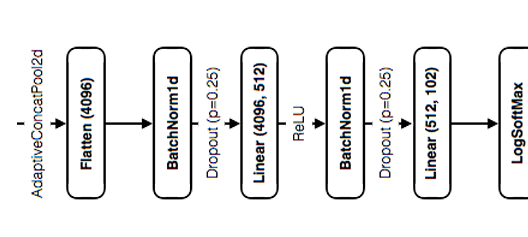
\includegraphics[width=.75\columnwidth]{resnet-50-2.png}
\caption{Alterações da Fast.ai na saída da Resnet-50}
\label{resnet50}
\end{center}
\end{figure}

Automaticamente, a biblioteca remove a camada final da Resnet-50 e adapta para o nosso problema onde a saída é a probabilidade de cada uma das 102 categorias\ref{resnet50}.


 
\subsection{Validação Cruzada}
Validação Cruzada (\textit{Cross Validation}) é uma técnica para criar uma base de validação a partir da base de treinamento. Em uma validação cruzada k-fold, a amostra original é aleatoriamente particionada em subamostra em \(k\) partes de igual tamanho, mutualmente exclusivas.  Depois do particionamento, uma das subamostras é utilizada para teste e as demais \(k-1\) para treinamento. Ao final de \(k\) interações temos 5 modelos treinados em bases diferentes.
% \begin{figure}[ht!]
% \begin{center}
% 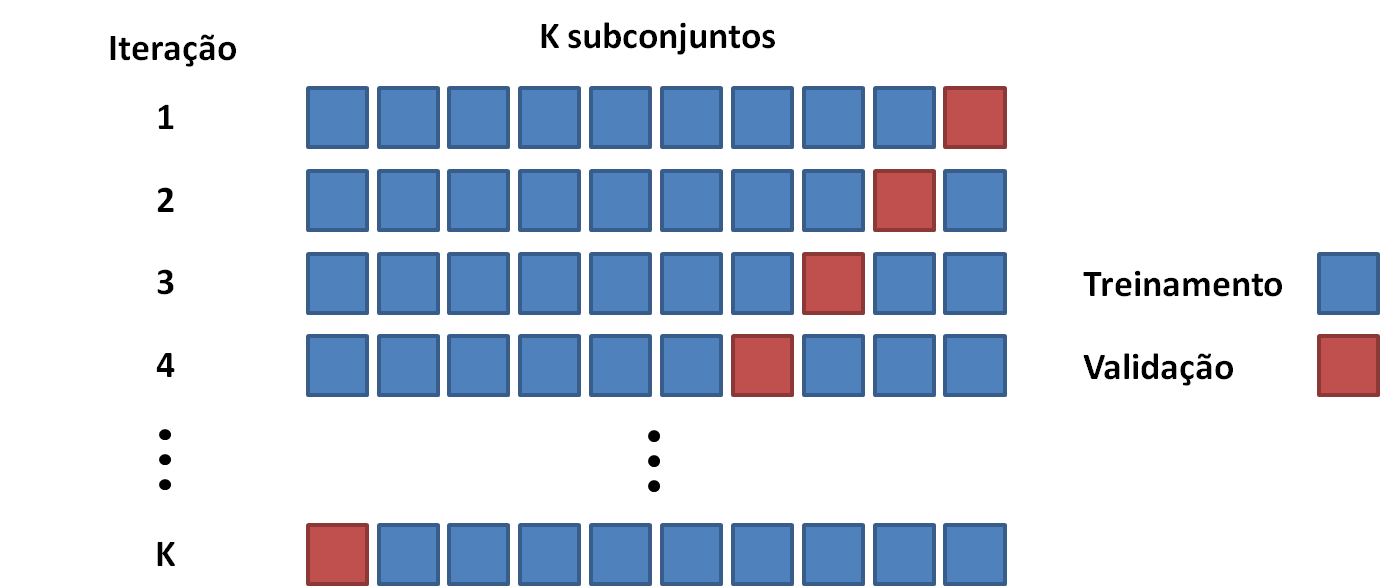
\includegraphics[width=.45\columnwidth]{k-fold.png}
% \caption{Validação cruzada k-fold}
% \end{center}
% \end{figure}
\subsection{Data Augmentation}
Uma outra forma de contornar o problema de falta de dados é adicionar dados falsos no conjunto de treinamento com características que sabemos serem similares aos dados reais. Para diversos problemas gerar dados falsos não é uma abordagem viável. Mas em problemas visuais, sabemos que podemos aplicar operações de translação, rotação, escala e alteração cromática em imagens e melhorar os resultados do treinamento.


\subsection{Otimização da Taxa de Aprendizado (Learning Rate)}

Modelos de RCPs são normalmente treinados usando um otimizador por gradiente descendente estocástico (\textit{Stochastic Gradient Descent} ou SGD). Há diversos tipos de otimizadores: Adam, RMSProp, Adagrad, etc. Todos permitem a definição da taxa de aprendizado (\textit{learning rate}), que é o quanto o otimizador deve mover os pesos na direção do gradiente para um determinado mini-batch.

Com uma taxa pequena, o treinamento é mais confiável, mas exige mais tempo e processamento para chegar a um valor mínimo da função de perda. Se a taxa é maior, anda-se a "passos mais largos", mas o treinamento pode não convergir ou até divergir. 

Para nos guiar na decisão da taxa mais adequada para o nosso problema, usamos a técnica descrita em\cite{cyclical}: começa-se a treinar a rede com uma taxa de aprendizado bem baixa e a aumentamos exponencialmente a cada batch. 

\begin{figure}
\centering
\subfloat {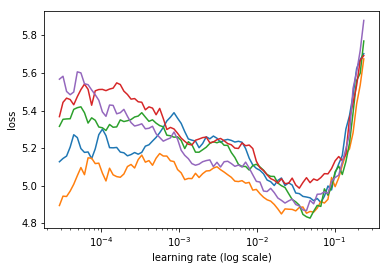
\includegraphics[width=4.2cm]{lr_1.png}}\hfil
\subfloat {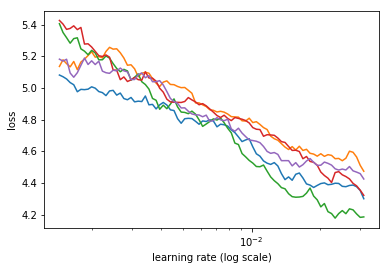
\includegraphics[width=4.2cm]{lr_2.png}}\hfil 
\caption{Procurando a taxa de aprendizado ótima}
\label{lr_find}
\end{figure}

\begin{figure}[ht!]
\begin{center}
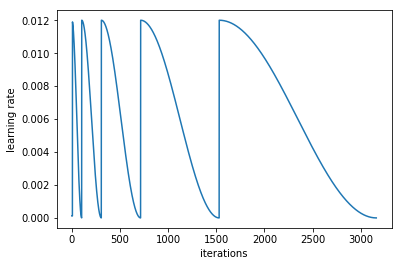
\includegraphics[width=.55\columnwidth]{cyclical_graph.png}
\caption{Variação cíclica da taxa de aprendizado}
\label{cycle}
\end{center}
\end{figure}

\begin{figure}[ht!]
\begin{center}
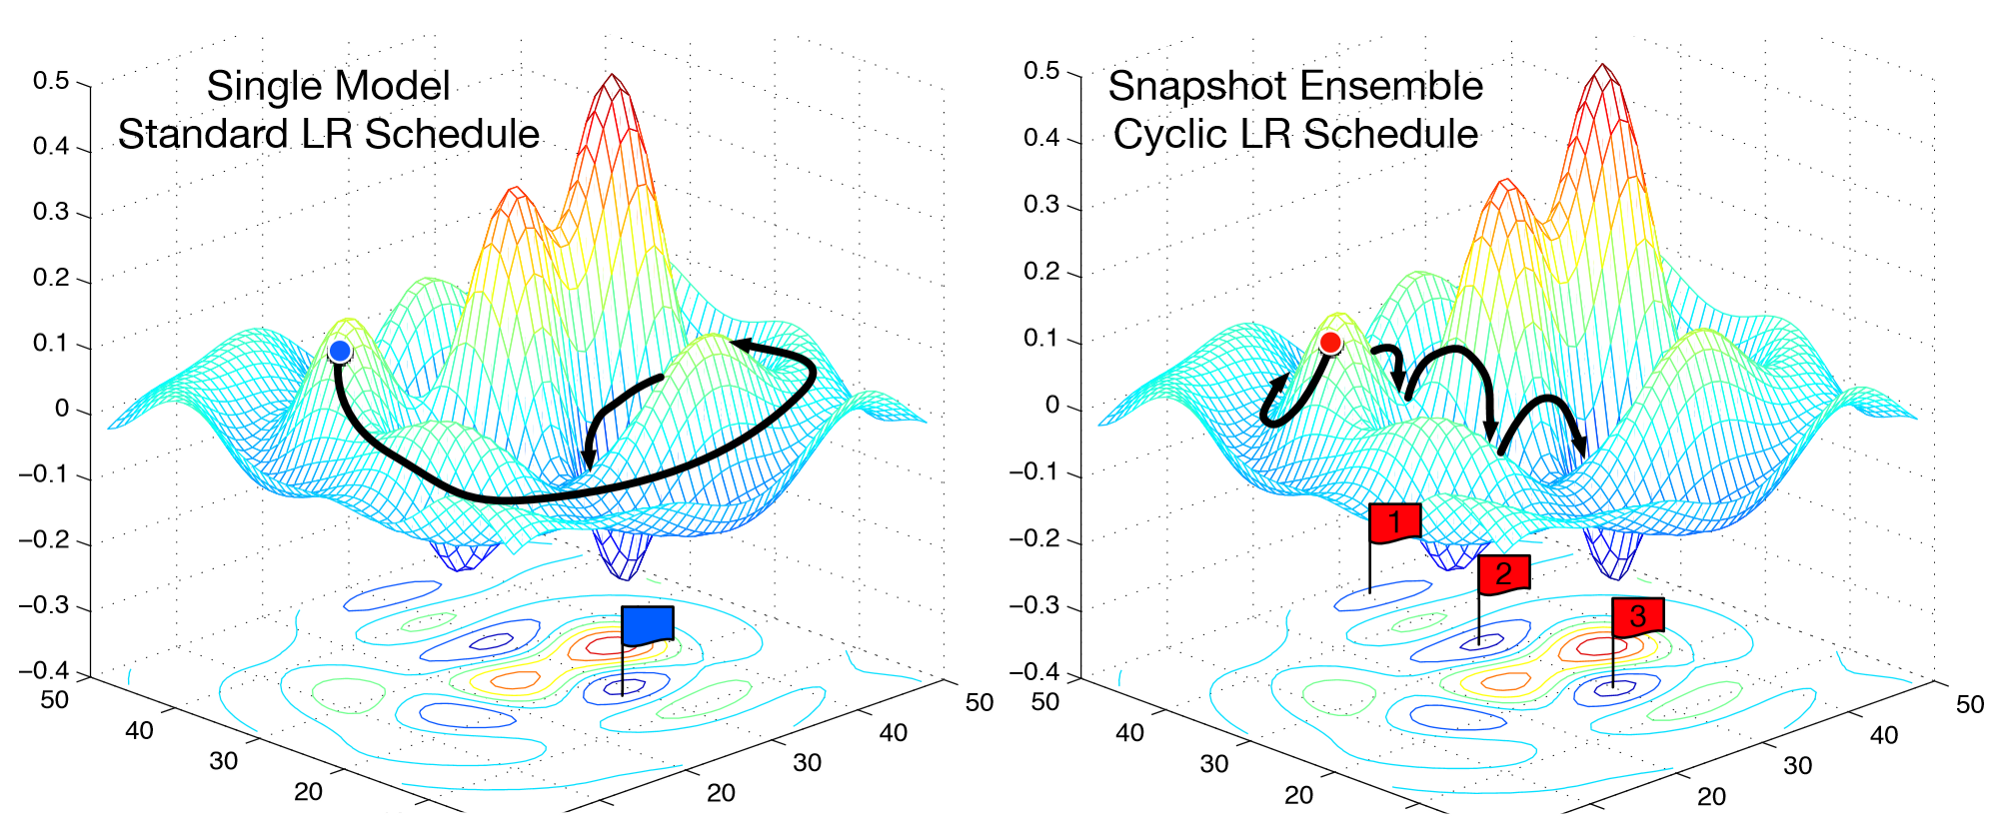
\includegraphics[width=\columnwidth]{minimos.png}
\caption{Variação cíclica permite encontrar diferentes mínimos\cite{cyclical}.}
\label{minimos}
\end{center}
\end{figure}

Na figura \ref{lr_find} vemos que de início a função de perda melhora muito lentamente, e depois começa a acelerar a partir de 0.001, até que por volta de 0.1 a taxa de aprendizado se torna grande demais e o treinamento diverge, ou seja, a perda começa a aumentar. 

A ideia é selecionar o ponto no gráfico com a perda mais rápida. No nosso exemplo, a perda diminui rapidamente na proximidade da taxa de aprendizado 0.012, que é a que decidimos usar. Selecionar uma boa taxa inicial para o treinamento é apenas o começo, a ideia mais interessante da técnica é como se altera a taxa de treinamento durante o treinamento.  O mais comum é definir uma taxa de decaimento, mas fugindo ao senso comum,\cite{cyclical} sugere uma variação cíclica em que a taxa de aprendizado pode sofrer aumentos repentinos. A figura \ref{cycle} mostra um gráfico com a função de variação da taxa de decaimento que usamos em nossos treinamentos.

A justificativa é facilmente entendida na figura \ref{minimos} do próprio artigo.  A maneira convencional nos ajuda a chegar em um mínimo da função de perda que pode ser local. Já usando uma variação cíclica, podemos chegar a vários mínimos diferentes, permitindo-se até obter um mínimo global, uma ideia que, apesar do artigo não mencionar, remonta a outra mais antiga, Otimização por Recozimento Simulado (Simulated Annealing Optimization)\cite{annealing}.

No projeto, rodamos as duas opções, com a taxa fixa em 0.012 por 30 épocas (single rate) e com a taxa cíclica (cyclical rate)\ref{cycle}.


\subsection{Otimizações em Tempo de Teste}

Em tempo de teste fizemos duas otimizações que se mostraram interessantes:
\begin{enumerate}
\item Test Time Augmentation: Em tempo de teste, para cada imagem do conjunto de dados de teste, aplicamos transformações de Data Augmentation e para definir a classe do objeto, calculamos a média de todas as predições desse conjunto "aumentado".  Para cada imagem de teste, geramos 4 imagens derivadas.
\item Test Time Model Average: Ao usar o k-fold para treinar os dados, em cada rodada temos 5 modelos treinados com 5 predições. Para cada imagem avaliada, tiramos a média das 5 predições.
\end{enumerate}


\section{Resultados}
Nesta seção apresentamos os resultados obtidos. Todos os dados podem ser acessados no repositório do projeto (\ref{repo}).

Quantitativamente, os resultados foram interessantes, como se pode ver na Tabela \ref{tabela}.
% Please add the following required packages to your document preamble:
% \usepackage{booktabs}
\begin{table}[]
\centering
\caption{Resultados quantitativos}
\label{tabela}
\begin{tabular}{@{}rrr@{}}
\toprule
            & \multicolumn{1}{c}{Single Rate} & \multicolumn{1}{c}{Cyclical Rate} \\ \midrule
Treinamento (s) & \(693.40\pm6.39\)& \(737.24\pm2.52\)                                  \\ \midrule
Predição (s)    & \(427.70\pm5.08\)&  \(435.08\pm0.88\)                                \\ \midrule
Acurácia  (\%)  & \(84.26\pm0.98\)  & \(85.13\pm0.74\)                              \\ \bottomrule
\end{tabular}
\end{table}

\subsection{Análise dos resultados}
Em face aos resultados obtidos, cabem algumas análises:
\begin{enumerate}
    \item A versão cíclica foi apenas 1\% melhor que a versão com taxa fixa e 6\% mais lenta. Esse resultado não nos permite dizer que comprovamos experimentalmente a superioridade da versão cíclica como descrito em \cite{annealing, fastai}. Um possível motivo pode ser o pequeno número de imagens de treinamento.
    \item Nosso melhor resultado, 85,13\% de acurácia, está a 8.9\% do recorde (93.42\%\cite{he}), entretanto, essa não é uma comparação justa, uma vez que o recorde foi obtido treinando-se com 30 imagens.
\end{enumerate}


\section{Discussão e Conclusões}
Neste trabalho, implementamos um algoritmos para reconhecimento de objetos para base Caltech 101. Utilizamos a arquitetura ResNet-50 pré-treinada com imagens da ImageNet e aplicamos otimizações de hiperparâmetros. A acurácia obtida com 5 imagens de treinamento foi 85,13\%. Acreditamos que esse resultado pode ser ainda melhorado explorando outras arquiteturas e 30 imagens por classe para treinamento. 

% \begin{figure}[htbp]
% \centerline{
\includegraphics{fig.jpg}}
% \caption{Example of a figure caption.}
% \label{fig}
% \end{figure}

\selectlanguage{brazilian}
\bibliographystyle{IEEEtran}
\bibliography{references}

\end{document}
